\appendix

\section{Data Pipeline: Buffer Size Profiling}
\label{app:buffer-profiling}

Training samples are drawn from an in-memory ring buffer that is asynchronously
refreshed from disk.  Because the buffer serves samples directly from RAM, disk
I/O is never a training-throughput bottleneck; the GPU is always the binding
constraint.  Buffer size therefore controls \emph{sample diversity} (how often
the same game/timestep pair is revisited before a slot refreshes) rather than
throughput.

Table~\ref{tab:buffer-profile} reports measurements on the NAO dataset
(88{,}239 players; see Section~\ref{sec:experiments}) for four buffer sizes.
Games are sampled proportional to the number of valid starting positions, which
biases the buffer towards long episodes ($\approx$18k frames on average).
The refresh fraction is 10\% per 60-second cycle.

\begin{table}[h]
\centering
\caption{Buffer profiling on NAO (horizon=128, context=4, NFS storage).
Reuse ratio = expected number of times a unique starting position is
sampled in one refresh cycle; lower is better.}
\label{tab:buffer-profile}
\begin{tabular}{rrrr rrrr}
\toprule
Buffer & Startup & RAM & Unique & \multicolumn{3}{c}{Reuse ratio @ GPU speed} \\
\cmidrule(lr){5-7}
size & (s) & (GB) & starts & 5k s/s & 20k s/s & 50k s/s \\
\midrule
  50 &  370 &  3.5 &    907{,}327 & 0.5$\times$ & 2.1$\times$ & 5.3$\times$ \\
 100 &  776 &  7.8 &  2{,}011{,}382 & 0.3$\times$ & 1.4$\times$ & 3.4$\times$ \\
 200 & 1623 & 16.8 &  4{,}336{,}761 & 0.3$\times$ & 1.0$\times$ & 2.6$\times$ \\
 500 & 4903 & 39.3 & 10{,}171{,}439 & 0.3$\times$ & 1.1$\times$ & 2.7$\times$ \\
\bottomrule
\end{tabular}
\end{table}

The reuse ratio is approximately \emph{constant} across buffer sizes: a larger
buffer yields proportionally more unique starts but also a proportionally longer
refresh cycle, so the ratio cancels.  The dominant tradeoff is therefore between
RAM usage and startup latency.  We use \texttt{buffer\_size=100} for all
experiments (7.8\,GB RAM, 13-minute startup, ${\le}$2$\times$ reuse at up to
20k samples/s).

\section{GPU Memory and Throughput: Encoder Variants}
\label{app:gpu-profiling}

We profile four encoder variants under both the LAM and LOM objectives
(\texttt{patch\_size=8}, \texttt{torch.compile}, \texttt{bfloat16}, 96\,GB GPU).
The \emph{Reconstruction} encoder ($d{=}256$, $L{=}4$, 311\,M total parameters)
uses pixel-level reconstruction; its dynamics head alone accounts for 268\,M
parameters (two heads of $\text{vocab\_size}\times P^2 = 8192\times 64$ each),
while the backbone contributes only 43\,M.  The three \emph{Latent} variants
predict a 512-dimensional EMA target latent, so their dynamics head is negligible
($<$0.3\,M); their parameter budgets differ solely in backbone depth and width:
\emph{Latent} matches the Reconstruction backbone ($d{=}256$, $L{=}4$);
\emph{Latent-medium} uses a wider backbone ($d{=}512$, $L{=}8$, ${\approx}$288\,M
trainable); and \emph{Latent-params} is parameter-matched to Reconstruction
($d{=}512$, $L{=}9$, ${\approx}$314\,M trainable).

Figure~\ref{fig:context_length} and Table~\ref{tab:pareto_lam} report the
memory--throughput Pareto frontier across context lengths for both objectives.

\begin{figure}[h]
\centering
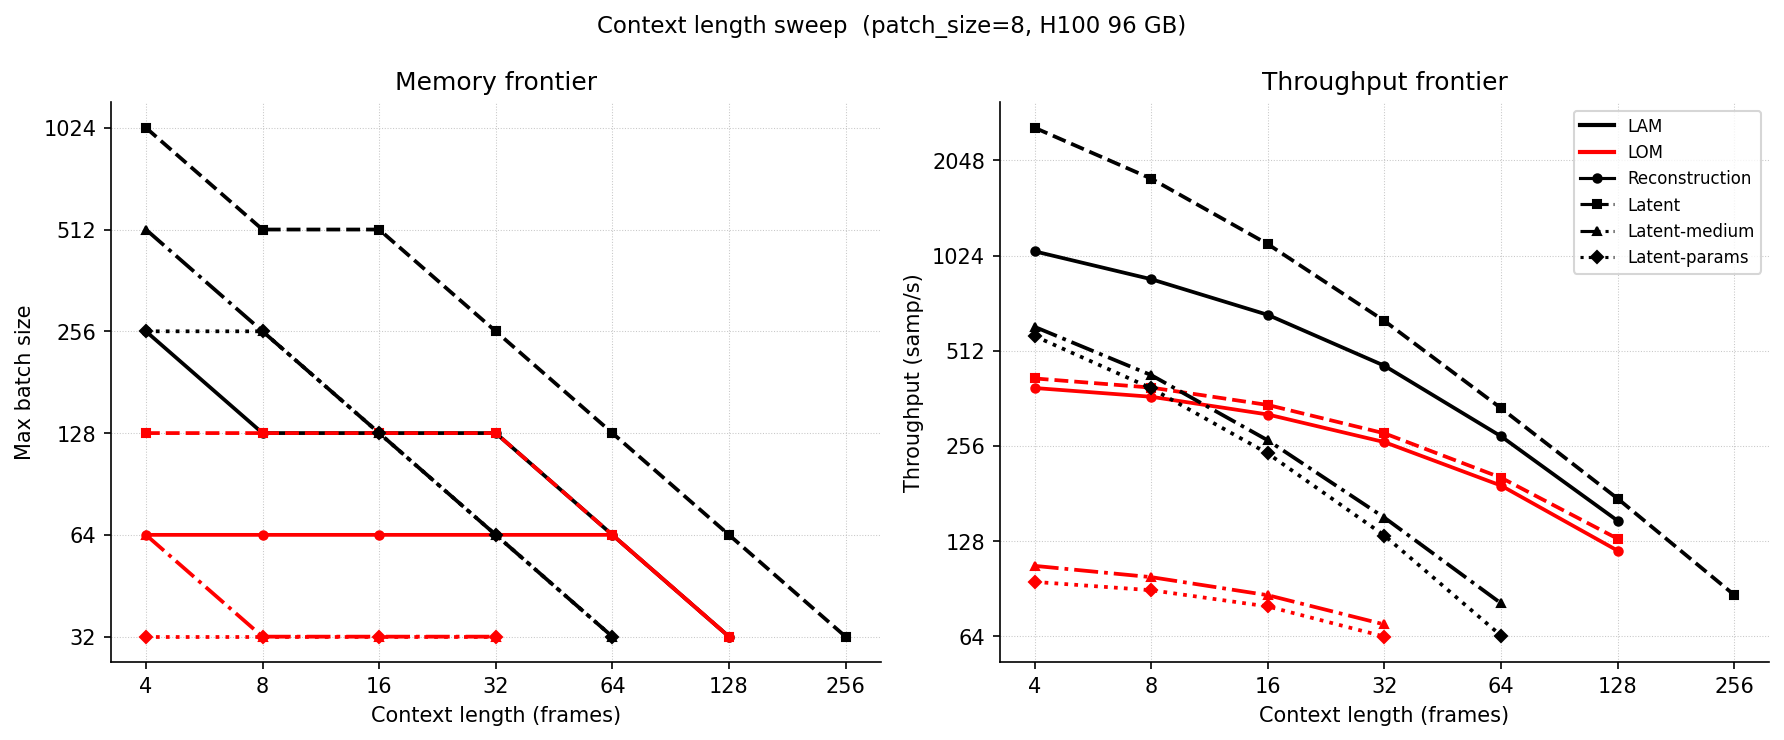
\includegraphics[width=\linewidth]{figures/context_length}
\caption{Context-length Pareto frontier on an 96\,GB GPU.
Black lines = LAM (horizon=1); red lines = LOM (horizon=128).
Line style encodes architecture: solid = Reconstruction, dashed = Latent,
dash-dot = Latent-medium, dotted = Latent-params.
\emph{Left}: largest fitting batch size per context length.
\emph{Right}: throughput (samples/s) at that batch size.}
\label{fig:context_length}
\end{figure}

\begin{table}[h]
\centering
\caption{LAM pareto results (\texttt{patch\_size=8}, compiled, 96\,GB GPU).
Max batch = largest batch size that fits in memory; samp/s at that batch.
``---'' = OOM at batch$=32$.}
\label{tab:pareto_lam}
\setlength{\tabcolsep}{4pt}
\begin{tabular}{r rr rr rr rr}
\toprule
 & \multicolumn{2}{c}{Reconstruction (311\,M)} & \multicolumn{2}{c}{Latent} & \multicolumn{2}{c}{Latent-medium (288\,M)} & \multicolumn{2}{c}{Latent-params (314\,M)} \\
\cmidrule(lr){2-3}\cmidrule(lr){4-5}\cmidrule(lr){6-7}\cmidrule(lr){8-9}
ctx & max b & samp/s & max b & samp/s & max b & samp/s & max b & samp/s \\
\midrule
  4 & $\ge$256 & 1264 & 2048 & 3547 & 1024 &  897 & 256 &  547 \\
  8 & $\ge$256 & 1053 & 1024 & 2231 &  512 &  562 & 256 &  381 \\
 16 & $\ge$256 &  796 &  512 & 1276 &  256 &  322 & 128 &  217 \\
 32 &  128 &  527 &  256 &  667 &  128 &  168 &  64 &  116 \\
 64 &  128 &  250 &  128 &  346 &   64 &   88 &  32 &   58 \\
128 &   64 &  167 &   64 &  178 &   32 &   45 & --- &  --- \\
256 &   32 &   86 &   32 &   88 &  --- &  --- & --- &  --- \\
\bottomrule
\end{tabular}
\end{table}

JEPA-compute matches STT's context reach (ctx$=256$ at batch$=32$) while
sustaining 3--4$\times$ higher throughput at short contexts: the pixel
reconstruction head in STT carries the same backbone compute but adds a
large logits tensor ($B \times H{\times}W \times \text{vocab}$) that caps
the fitting batch size.  JEPA-params, despite matching STT in total parameter
count, exhausts memory earlier because its 12-layer backbone accumulates
proportionally more activation memory; its DynamicsModel head is negligible.
This makes JEPA-compute the most memory-efficient choice for long-context
training, and JEPA-medium the natural candidate when additional backbone
capacity is warranted without the overhead of pixel reconstruction.

Tables~\ref{tab:pareto_lom} and~\ref{tab:horizon_lom} summarise the numerical results.

\begin{table}[h]
\centering
\caption{LOM context pareto (\texttt{patch\_size=8}, horizon=128, compiled, 96\,GB GPU).
``---'' = OOM at batch$=32$.}
\label{tab:pareto_lom}
\setlength{\tabcolsep}{5pt}
\begin{tabular}{r rr rr rr}
\toprule
 & \multicolumn{2}{c}{Reconstruction-LOM (311\,M)} & \multicolumn{2}{c}{Latent-LOM} & \multicolumn{2}{c}{Latent-medium-LOM (288\,M)} \\
\cmidrule(lr){2-3}\cmidrule(lr){4-5}\cmidrule(lr){6-7}
ctx & max b & samp/s & max b & samp/s & max b & samp/s \\
\midrule
  4 &  64 & 220 &  64 & 155 &  32 &  41 \\
  8 &  64 & 204 &  64 & 150 &  32 &  39 \\
 16 &  64 & 183 &  64 & 137 &  32 &  35 \\
 32 &  64 & 148 &  64 & 116 & --- & --- \\
 64 &  32 & 103 &  64 &  91 & --- & --- \\
128 &  32 &  66 &  32 &  60 & --- & --- \\
\bottomrule
\end{tabular}
\end{table}

\begin{figure}[h]
\centering
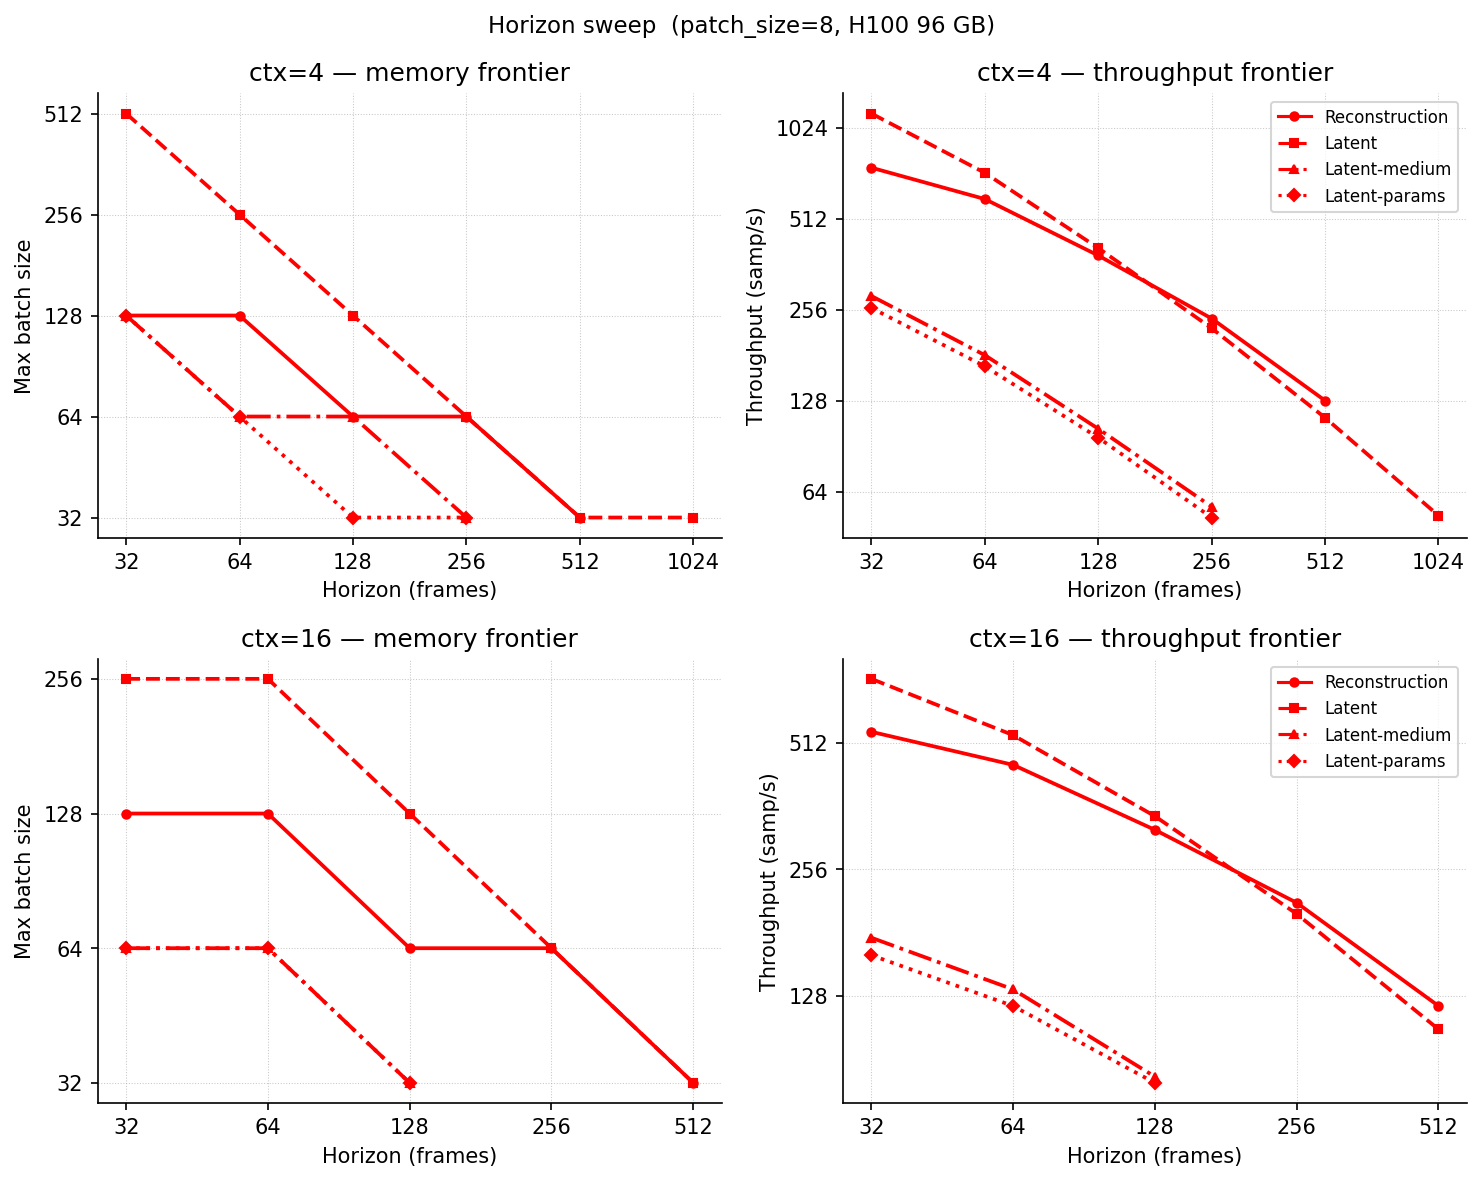
\includegraphics[width=\linewidth]{figures/horizon}
\caption{LOM horizon sweep at fixed ctx=4.
Line style encodes architecture: solid = Reconstruction, dashed = Latent,
dash-dot = Latent-medium, dotted = Latent-params.
\emph{Left}: largest fitting batch size per horizon.
\emph{Right}: throughput (samples/s) at that batch size.}
\label{fig:horizon_lom}
\end{figure}

\begin{table}[h]
\centering
\caption{Maximum affordable horizon (batch$\ge 32$) at fixed ctx=4.
``---'' = OOM at batch$=32$ even for the shortest horizon tested.}
\label{tab:horizon_lom}
\setlength{\tabcolsep}{6pt}
\begin{tabular}{r rrr}
\toprule
horizon & Reconstruction-LOM & Latent-LOM & Latent-medium-LOM \\
\midrule
  4 & 512 & 256 & 128 \\
 32 & 512 & 256 &  64 \\
 64 & 512 & 256 &  32 \\
\bottomrule
\end{tabular}
\end{table}

The Reconstruction encoder is dominated by its two pixel dynamics heads (268\,M of 311\,M total),
which cap the fitting batch size early but are memory-independent of horizon length.
The Latent variants carry negligible dynamics heads but pay for EMA target encoders that must
process the full horizon sequence, limiting maximum horizon more than Reconstruction at equivalent
context.  Latent-params-LOM exhausts the 96\,GB budget at every context length and is not a
viable training configuration at this scale.
